\documentclass[a4paper]{article}

\usepackage{graphicx}
\graphicspath{{./images/}}

\usepackage[T1]{fontenc}
\usepackage{textcomp}
\usepackage{amsmath, amssymb}
\usepackage{enumitem}
\usepackage{import}
\usepackage{xifthen}
\usepackage{transparent}
\usepackage[affil-it]{authblk}

\title{COMP 346: Operating Systems \\
 Theory Assignment no.1}
 \author{Duc Nguyen}

 \affil{Gina Cody School of Computer Science and Software Engineering \\
    Concordia University, Montreal, QC, Canada}

\date{Winter 2020}

\begin{document}

\begin{titlepage}
\maketitle
\end{titlepage}

\newpage
\tableofcontents
\newpage

\section{Essential definitions of OS}
\subsection{What is an operating system?}

\textbf{Problem:}
What is an operating system? What are the main purposes of an operating system?

\textbf{Answer:}
In general, Operating System is a program that acts as an intermediary between a user of a computer and the computer hardware. However, there is actually no universally accepted definition for OS, it varies from different points of view.
\\
Main purposes of an OS
\begin{itemize}
    \item Execute user programs and make solving user problems easier
    \item Make the computer system convenient to use
    \item Use the computer hardware in an efficient manner.
\end{itemize}

\subsection{Essential properties of operating systems}
Define the essential properties of the following types of operating systems:
\subsubsection{Batch}
Batch processing (or multiprogramming) is a technique in which the similar programs will be grouped together in a batch before the process starts. Jobs are scheduled to be processed in the order of submission (first come first served basic) and one job at a time. Ultimately, Batch system can be considered as a type of Serial processing.

\begin{figure}[ht]
    \centering
    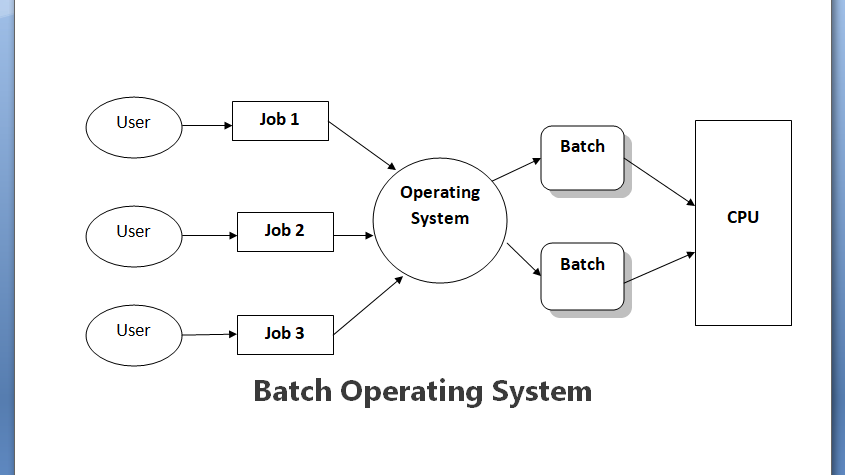
\includegraphics[scale=0.5]{BatchSystem}
    \caption{Batch System}
\end{figure}

\begin{itemize}
    \item
    \textbf{Advantages:} Performance is increased when switching between tasks since the CPU already decides the next job to be executed before the current job get done (Scheduled before hand)
    \item
    \textbf{Disadvantages:} A job depends on another job's execution time. Thus, if a job gets into an infinite loop, the pending jobs will be stuck.
\end{itemize}

\subsubsection{Time Sharing}
Time Sharing (or multi-tasking) system is a system that allows multiple jobs running at the same time by sharing the CPU among them. Time Sharing aims to minimize response time of a process instead of focusing on the processor use of the process. Normally, the response time should be reduced to $< 1$ second. CPU is scheduled when there are several jobs ready to run at a time. It is also the first model for multiprocessing.

\begin{itemize}
    \item \textbf{Advantages:}
        \begin{itemize}
            \item Minimize the response time of the system
            \item Avoid infinite wait time when a process gets into infinite loop.
        \end{itemize}
    \item \textbf{Disadvantages:}
        \begin{itemize}
            \item Security concerns since there are more users using the CPU.\\
        \end{itemize}
\end{itemize}

\begin{figure}[ht]
\centering
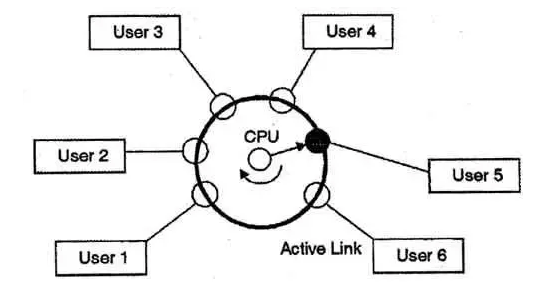
\includegraphics[scale=0.5]{time-sharingSystem}
\caption{Time Sharing System on Unix}
\end{figure}

\subsubsection{Dedicated}
A dedicated system is a system that is specifically designed for a specific task. Users of dedicated systems have dedicated resources but frequently use shard resources from \textbf{server}.

\subsubsection{Real time}
Real time system is often embedded system.The system should have response in a time constraint. It is usually designed for a special purpose such as flight control system.


\subsection{Circumstances to use time-sharing system}
\textbf{Problem:}
Under what circumstances would a user be better of using a time-sharing system rather than a PC or single-user workstation?\\
\textbf{Answer:}
User should prefer a time-sharing system rather than a single-user workstation when there is a need for collaborate or simply there are several other users want to use the system. The amount of task also counts as a factor. When the task is large, time-sharing would be much more efficient. Time-sharing is also preferable in case many users want to access resources at the same time.
A personal computer (single-user workstation) should only be used when the task needs to be executed is small enough.

\newpage
\section{Single programmed versus Multiprogrammed OS}
\textbf{Problem:}
Consider a computer system with a single-core processor. There are two processes to run in the system: $P_1$ and $P_2$.
Process $P_1$ has a life cycle as follows: CPU burst time of 15 units, followed by I/O burst time of minimum 10 units, followed by CPU burst time of 10 units.
Process $P_2$ has the following life cycle: CPU burst time of 10 units, followed by I/O burst time of minimum 5 units, followed by CPU burst time of 15 units.

\subsection{Single programmed Operating System}
\textbf{Problem:}
Considering a \textit{single programmed} operating system, what is the minimal total time required to complete executions of the two processes?
You should explain your answer with a diagram
\\
\textbf{Answer:}
Since the operating system is of single programmed, the CPU only can execute one process at a time\\
$\implies$\textbf{Minimal total time:} $P_1 time + P_2 time = (15 + 10 + 10) + (10 + 5 + 15) = 65$ units

\begin{figure}[ht]
    \centering
    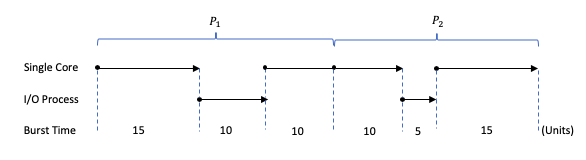
\includegraphics[scale=0.5]{singlecoreProcess}
    \caption{Single core processing}
\end{figure}

\subsection{Multiprogrammed Operating system}
\textbf{Problem:}
Now considering a \textit{multiprogrammed} operating system, what is the minimal total time required to complete executions of the two processes?
You should explain your answer with a diagram
\\
\textbf{Answer:}
The operating system is multiprogrammed $\implies$ The CPU can execute multiple processes at once. Therefore, both $P_1 and P_2$ can start at the same time.
\\
$\implies$\textbf{Minimal total time:} $15 + 10 + 10 = 35$ units

\begin{figure}[ht]
    \centering
    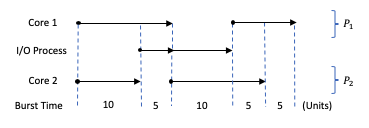
\includegraphics[width=150mm,scale=0.8]{multicoreProcess}
    \caption{Multi core processing}
\end{figure}

\subsection{Throughput}
\textbf{Problem:}
\textit{Throughput} is defined as the number of processes (tasks) completed per unit time.
Following this definition, calculate the throughputs for parts \textbf{1} and \textbf{2} above. How does multiprogramming affect throughput? Explain your answer.
\\
\textbf{Answer:}
\begin{itemize}
    \item\textbf{Throughput part 1:} $\frac{2}{65} = 0.0307$ (processes)
    \item\textbf{Throughput part 2:} $\frac{2}{35} = 0.0571$ (processes)
\end{itemize}


\newpage
\section{Device interrupts}
\subsection{Interrupts versus Polling}
\textbf{Problem}
What is the performance advantage in having device drivers and devices synchronize by means of device interrupts, rather than by polling (i.e., device driver keeps on polling the device to see if a specific event has occurred)?
Under what circumstances can polling be advantageous over interrupts?
\\
\textbf{Answer:}

\subsection{Posibility of using DMA controller with system does not support interrupts}
\textbf{Problem:}
Is it possible to use a DMA controller if the system does not support interrupts?
\\
\textbf{Answer:}


\subsection{Context Switch problems}
\textbf{Problem:}
The procedure \textit{ContextSwitch} is called whenever there is a switch in context from a running program A to another program B.
 The procedure is a straightforward assembly language routine that saves and restores registers, and must be atomic.
 Something disastrous can happen if the routine ContextSwitch is not atomic.

 \begin{enumerate}
     \item Explain why \textit{ContextSwitch} must be atomic, possibly with an example.
    \item Explain how the atomicity can be achieved in practice.
 \end{enumerate}
 \textbf{Answer:}

 \newpage
\section{System mode and User mode}
\subsection{Performing I|O by User or Kernel?}
\textbf{Problem:}
If a user program needs to perform I/O, it needs to trap the OS via a system call that transfers control to the kernel. The kernel performs I/O on behalf of the user program.
However, systems calls have added overheads, which can slow down the entire system. In that case, why not let user processes perform I/O directly, without going through the kernel?
\\
\textbf{Answer:}


\subsection{Scenario: User tricks the OS to run monitor mode}
\textbf{Problem:}
Consider a computer running in the user mode.
It will switch to the monitor mode whenever an interrupt or trap occurs, jumping to the address determined from the interrupt vector.
\begin{enumerate}
    \item A smart, but malicious, user took advantage of a certain serious loophole in the computer's protection mechanism, by which he could make run his own user program in the monitor mode! This can cause disastrous effects.
    What could have he possibly done to achieve this? What disastrous effects could it cause?
    \item Suggest a remedy for the loophole.
\end{enumerate}
\textbf{Answer:}

\newpage
\section{Multi processes}
\textbf{Problem:}
Suppose that a multiprogrammed system has a load of N processes with individual execution times of $t_1, t_2, \ldots, t_N$. Answer the following questions:
\begin{enumerate}
    \item How would it be possible that the time to complete the N processes could be as small as: \textit{maximum} ($t_1, t_2, \ldots,t_N$)?
    \item How would it be possible that the total execution time, $T > t_1 + t_2 +\ldots+ t_N$? In other words, what would cause the total execution time to exceed the sum of individual process execution times?
\end{enumerate}
\textbf{Answer:}


\newpage
\section{Privileged instructions}
\textbf{Problem:}
Which of the following instructions should be privileged? Explain why.
\begin{enumerate}[label=\roman*.]
    \item Read the system clock
    \item Clear memory
    \item Reading from user space
    \item Writing to user space
    \item Copy from one register to another
    \item Turn off interrupts
    \item Switch from user to monitor mode.
\end{enumerate}
\textbf{Answer:}

\newpage
\section{Design Network Operating System versus Distributed Operating System}
\textbf{Problem:}
Assume you are given the responsibility to design two OS systems, a Network Operating System and a Distributed Operating System. Indicate the primary differences between these two systems.
Additionally, you need to indicate if there any possible common routines between these systems?
If yes, indicate some of these routines. If no, explain why common routines between these two particular systems do not make sense.
\\
\textbf{Answer:}


\end{document}
